\begin{task}
\TT{Oblicz moc sygnału okresowego $f(t)=A + B \cdot sin\left(\frac{2\pi}{T}\cdot t \right )$ przedstawionego na rysunku:}{Compute the average power for the following periodic signal $f(t)=A + B \cdot sin\left(\frac{2\pi}{T}\cdot t \right )$ given below:}

\begin{figure}[H]
\centering
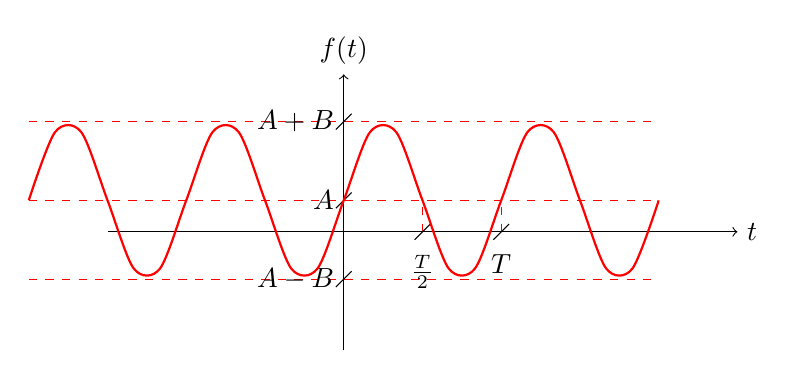
\begin{tikzpicture}
  \draw[->] (-3.0,+0.0) -- (+5.0,+0.0) node[right] {$t$};
  \draw[->] (+0.0,-1.5) -- (+0.0,+2.0) node[above] {$f(t)$};
  \draw[-,red, dashed] (-4.0,+1.4) -- (+4.0,+1.4);
  \draw[-,red, dashed] (-4.0,-0.6) -- (+4.0,-0.6);
  \draw[-,red, dashed] (-4.0,+0.4) -- (+4.0,+0.4);
  \draw[-,red, dashed] (+1.0,+0.0) -- (+1.0,+0.4);
  \draw[-,red, dashed] (+2.0,+0.0) -- (+2.0,+0.4);
  %\draw[-] (-1.0-0.1,-0.1)--(-1.0+0.1,0.1) node[midway, below, outer sep=10pt,align=center] {$-\frac{T}{2}$};
  \draw[-] (+1.0-0.1,-0.1)--(+1.0+0.1,0.1) node[midway, below, outer sep=5pt] {$\frac{T}{2}$};
  \draw[-] (+2.0-0.1,-0.1)--(+2.0+0.1,0.1) node[midway, below, outer sep=5pt] {$T$};
  \draw[-] (-0.1,+1.4-0.1)--(+0.1,+1.4+0.1) node[midway, left] {$A+B$};
  \draw[-] (-0.1,+0.4-0.1)--(+0.1,+0.4+0.1) node[midway, left] {$A$};
  \draw[-] (-0.1,-0.6-0.1)--(+0.1,-0.6+0.1) node[midway, left] {$A-B$};
  
  \draw[scale=1.0,domain=-4.0:4.0,smooth,variable=\x,red,thick] plot ({\x},{0.4+ sin(\x*180.0/3.141592*2*3.141592/2.0)});

\end{tikzpicture}
\end{figure}

\TT{Moc sygnału okresowego wyznaczamy ze wzoru:}{The average power for periodic signals is defined by:}

\begin{equation}
P=\frac{1}{T} \cdot \int_{T}^{}\left|f(t)\right|^2 \cdot dt
\end{equation}

\TT{Podstawiamy do wzoru na moc wzór naszej funkcji :}{In our case we get:}

\begin{align*}
P&=\frac{1}{T} \cdot \int_{T}^{}\left|f(t)\right|^2 \cdot dt=\\
 &=\frac{1}{T} \cdot \int_{0}^{T}\left|A + B \cdot sin\left(\frac{2\pi}{T}\cdot t \right) \right|^2 \cdot dt=\\ 
 &=\frac{1}{T} \cdot \int_{0}^{T}\left(A + B \cdot sin\left(\frac{2\pi}{T}\cdot t \right) \right)^2 \cdot dt=\\ 
 &=\frac{1}{T} \cdot \int_{0}^{T}\left(A^2 + 2\cdot A \cdot B \cdot sin\left(\frac{2\pi}{T}\cdot t \right) + B^2 \cdot sin^2\left(\frac{2\pi}{T}\cdot t \right) \right) \cdot dt=\\
 &=\frac{1}{T} \cdot \left( \int_{0}^{T}A^2 \cdot dt + \int_{0}^{T} 2\cdot A \cdot B \cdot sin\left(\frac{2\pi}{T}\cdot t \right) \cdot dt + \int_{0}^{T} B^2 \cdot sin^2\left(\frac{2\pi}{T}\cdot t \right)  \cdot dt \right)=\\
 &=\frac{A^2}{T} \cdot \int_{0}^{T} dt + \frac{2\cdot A \cdot B}{T} \cdot \int_{0}^{T} sin\left(\frac{2\pi}{T}\cdot t \right) \cdot dt + \frac{B^2}{T} \cdot \int_{0}^{T}  sin^2\left(\frac{2\pi}{T}\cdot t \right)  \cdot dt=\\
 &=\begin{Bmatrix*}[l]
 z=\frac{2\pi}{T} \cdot t\\
 dz = \frac{2\pi}{T} \cdot dt & dt = \frac{dz}{\frac{2\pi}{T}} =\frac{T}{2\pi} \cdot dz 
 \end{Bmatrix*}=\\
 &=\frac{A^2}{T} \cdot \left. t \right|_{0}^{T} + \frac{2\cdot A \cdot B}{T} \cdot \int_{0}^{T} sin\left(z \right) \cdot \frac{T}{2\pi} \cdot dz + \frac{B^2}{T} \cdot \int_{0}^{T} \frac{1}{2} \cdot \left(1 - cos\left(2 \cdot \frac{2\pi}{T}\cdot t \right) \right)  \cdot dt=\\
 &=\frac{A^2}{T} \cdot \left( T - 0 \right) + \frac{2\cdot A \cdot B}{T} \cdot \frac{T}{2\pi} \cdot \int_{0}^{T} sin\left(z \right) \cdot dz + \frac{B^2}{T} \cdot \frac{1}{2} \cdot \int_{0}^{T} \left(1 - cos\left(2 \cdot \frac{2\pi}{T}\cdot t \right) \right)  \cdot dt=\\
 &=\frac{A^2}{T} \cdot T + \frac{A \cdot B}{\pi} \cdot \left( \left.-cos\left(z \right)\right|_{0}^{T}  \right) + \frac{B^2}{2 \cdot T} \cdot \left( \int_{0}^{T} 1 \cdot dt - \int_{0}^{T} cos\left(2 \cdot \frac{2\pi}{T}\cdot t \right)  \cdot dt \right)=\\
 &=\begin{Bmatrix*}[l]
 w=2\cdot \frac{2\pi}{T} \cdot t\\
 dw = 2\cdot \frac{2\pi}{T} \cdot dt & dt = \frac{dw}{\frac{4\pi}{T}} =\frac{T}{4\pi} \cdot dw 
 \end{Bmatrix*}=\\
 &=A^2 + \frac{A \cdot B}{\pi} \cdot \left( \left.-cos\left(\frac{2\pi}{T} \cdot t \right)\right|_{0}^{T}  \right) + \frac{B^2}{2 \cdot T} \cdot \left( \left. t \right|_{0}^{T} - \int_{0}^{T} cos\left(w \right)  \cdot \frac{T}{4\pi} \cdot dw \right)=\\
 &=A^2 + \frac{A \cdot B}{\pi} \cdot  \left(-cos\left(\frac{2\pi}{T} \cdot T \right)+cos\left(\frac{2\pi}{T} \cdot 0 \right)\right) + \frac{B^2}{2 \cdot T}  \cdot \left( \left(T - 0 \right) - \frac{T}{4\pi} \cdot \int_{0}^{T} cos\left(w \right)  \cdot dw \right)=\\
 &=A^2 + \frac{A \cdot B}{\pi} \cdot  \left(-cos\left(2\pi \right)+cos\left(0 \right)\right) + \frac{B^2}{2 \cdot T}  \cdot \left( T - \frac{T}{4\pi} \cdot \left. -sin\left(w \right)  \right|_{0}^{T} \right)=\\
 &=A^2 + \frac{A \cdot B}{\pi} \cdot  \left(-1+1\right) + \frac{B^2}{2 \cdot T}  \cdot \left( T + \frac{T}{4\pi} \cdot \left. sin\left(2\cdot \frac{2\pi}{T}\cdot t \right)  \right|_{0}^{T} \right)=\\
 &=A^2 + \frac{A \cdot B}{\pi}\cdot 0 + \frac{B^2}{2 \cdot T} \cdot \left( T + \frac{T}{4\pi} \cdot \left( sin\left(2\cdot \frac{2\pi}{T}\cdot T \right) - sin\left(2\cdot \frac{2\pi}{T}\cdot 0 \right) \right) \right)=\\
 &=A^2 + \frac{B^2}{2 \cdot T}  \cdot \left( T + \frac{T}{4\pi} \cdot \left( sin\left(4\pi \right) - sin\left( 0 \right) \right) \right)=\\
 &=A^2 + \frac{B^2}{2 \cdot T}  \cdot \left( T + \frac{T}{4\pi} \cdot \left( 0 - 0 \right) \right)=\\
 &=A^2 + \frac{B^2}{2 \cdot T}  \cdot \left( T \right)=\\
 &=A^2 + \frac{B^2}{2}
\end{align*}

\TT{Moc sygnału wynosi $A^2 + \frac{B^2}{2}$.}{The average power equals to $A^2 + \frac{B^2}{2}$.}
\end{task}